\clearpage
\section{GEOMETRIC PRELIMINARIES}
A \textbf{singular $n$-cube} in $A\subset \F{R}^n$ is a continuous function 
$c:[0,1]^n\to A$ (here $[0,1]^n$ denotes the $n$-fold product $[0, 1]\times\cdots\times[0,1]$).
We let $\F{R}^0$ and $[0,1]^0$ both denote $\{0\}$. A singular
0-cube in $A$ is then a function $f:\{0\}\to A$ or, what amounts to
the same thing, a point in $A$. A singular 1-cube is often
called a curve. A particularly simple, but particularly
important example of a singular $n$-cube in $\F{R}^n$ is the standard
$n$-cube $I^n:[0,1]^n\to\F{R}^n$ defined by $I^n(x) = x$ for $x\in[0,1]^n$.

We shall need to consider formal sums of singular $n$-cubes in
$A$ multiplied by integers, that is, expressions like
\begin{align*}
    2c_1 + 3c_2 - 4c_3
\end{align*}

where $c_1,c_2,c_3$ are singular $n$-cubes in $A$. Such a finite sum of singular 
$n$-cubes with integer coefficients is called an \textbf{$n$-chain} in $A$. In particular 
a singular $n$-cube $c$ is also considered as an $n$-chain $1\cdot c$. It is clear how 
$n$-chain can be added, and multiplied by integers. For example 
\begin{align*}
    2(c_1+3c_4) + (-2)(c_1+c_3+c_2) = - 2c_2 - 2c_3 + 6c_4
\end{align*}

(A rigorous exposition of this formalism is presented in Problem 4-22.)

For each singular $n$-chain $c$ in $A$ we shall define an $(n-1)$-chain in $A$ called the boundary 
of $c$ and denoted $\partial c$. The boundary of $I^2$, for example, might be defined as the sum of
four singular 1-cubes arranged counterclockwise around the boundary of $[0,1]^2$, as indicated in 
Figure \ref{Fig 4-4}(a). It is actually much more convenient to define $\partial I^2$ as the sum, with
the indicated coefficients, of the four singular 1-cubes shown in Figure \ref{Fig 4-4}(b). The precise 
definition of ar requires some preliminary notions. For each $i$ with $1 \le i\le n$ we define
two singular $(n-1)$-cubes $I^n_{(i,0)}$ and $l^n_{(i,l)}$ as follows. If $x\in[0,1]^{n-1}$, then 
\begin{align*}
    I^n_{(i,0)}(x) 
    & = I^n(x^1,\cdots,x^{i-1},0,x^i,\cdots,x^{n-1}) \\
    & = (x^1,\cdots,x^{i-1},0,x^i,\cdots,x^{n-1})\\
    I^n_{(i,1)}(x)
    & = I^n(x^1,\cdots,x^{i-1},1,x^i,\cdots,x^{n-1}) \\
    & = (x^1,\cdots,x^{i-1},1,x^i,\cdots,x^{n-1})
\end{align*}

\begin{figure}[!htb]
    \centering
    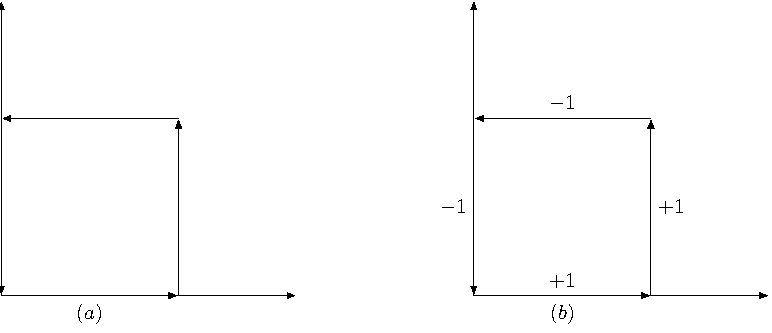
\includegraphics[width=.75\linewidth]{./pics/Fig4-4.pdf}
    \caption{}
    \label{Fig 4-4}
\end{figure}

We call $I^n_{(i,0)}$ the $(i,0)$-face of $I^n$ and $I^n_{(i,1)}$ the $(i,1)$-face of $I^n$.
(Figure \ref{Fig 4-5}). We then define 
\begin{align*}
    \partial I^n = \sum_{i=1}^n \sum_{\alpha=0,1}(-1)^{i+\alpha}I^n_{(i,\alpha)}
\end{align*}

For a general singular $n$-cube $c:[0,1]^n\to A$ we first define the $(i,\alpha)$-face,
\begin{align*}
    c_{(i,\alpha)} = c\circ I^n_{(i,\alpha)}
\end{align*}

and then define 
\begin{align*}
    \partial c = \sum_{i=1}^n \sum_{\alpha=0,1}(-1)^{i+\alpha}c_{(i,\alpha)}
\end{align*}

Finally we define the boundary of an $n$-chain $\sum_{}^{}{a_ic_i}$ by 
\begin{align*}
    \partial \sum_{}^{}{a_ic_i} = \sum_{}^{}{a_i\partial c_i}
\end{align*}

Although these few definitions suffice for all applications in
this book, we include here the one standard property of $\partial$.

\begin{figure}[!htb]
    \centering
    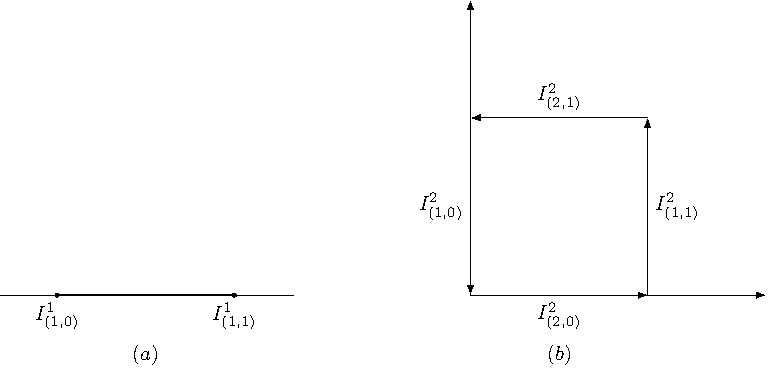
\includegraphics[width=.75\linewidth]{./pics/Fig4-5.pdf}
    \caption{}
    \label{Fig 4-5}
\end{figure}

\begin{theorem}
    If $c$ is an $n$-chain in $A$, then $\partial(\partial c) = 0$. Briefly, 
    $\partial^2 = 0$.
\end{theorem}

\begin{proof}
    Let $i\le j$ and consider $(I^n_{i,\alpha})_{(j,\beta)}$. If $x\in [0,1]^{n-2}$,
    then, remembering the definition of the $(j,\beta)$-face of a singular $n$-cube, we have 
    \begin{align*}
        (I^n_{(i,\alpha)})_{(j,\beta)}(x) 
        & = I^n_{(i,\alpha)}(I^{n-1}_{(j,\beta)}(x))\\
        & = I^n_{(i,\alpha)}(x^1,\cdots,x^{j-1},\beta,x^j,\cdots,x^{n-2}) \\
        & = I^{{n}}(x^{1},\cdots,x^{{i}-1},\alpha,x^{{i}},\cdots,x^{{j}-1},{\beta},x^{{j}},\cdots,x^{{n}-2})
    \end{align*}

    Similarly
    \begin{align*}
        (I^n_{(j+1,\beta)})_{(i,\alpha)}(x) 
        & = I^n_{(j+1,\beta)}(I^{n-1}_{(i,\alpha)}(x))\\
        & = I^n_{(j+1,\beta)}(x^1,\cdots,x^{i-1},\alpha,x^i,\cdots,x^{n-2}) \\
        & = I^{{n}}(x^{1},\cdots,x^{{i-1}},\alpha,x^{i},\cdots,x^{{j}-1},{\beta},x^{{j}},\cdots,x^{{n}-2})
    \end{align*}

    Thus $(I_{(i,\alpha)}^n)_{(j,\beta)}=(I_{(j+1,\beta)}^n)_{(i,\alpha)}$ for $i\le j$.
    (It may help to verify this in Figure 4-5.) It follows easily for any singular
    $n$-cube $c$ that $(c_{(i,\alpha)})_{(j,\beta)}=(c_{(j+1,\beta)})_{(i,\alpha)}$ when $i\le j$.
    Now
    \begin{align*}
        \partial(\partial c)
        & = \partial\left(\sum_{i=1}^n\sum_{\alpha=0,1}(-1)^{i+\alpha}c_{(i,\alpha)}\right) \\
        & = \sum_{i=1}^{n}\sum_{\alpha=0,1}\sum_{j=1}^{n-1}{\sum_{\beta=0,1}^{}{(-1)^{i+\alpha+j+\beta}(c_{(i,\alpha)})_{(j,\beta)}}}
    \end{align*} 

    In this sum $(c_{(i,\alpha)})_{(j,\beta)}$ and $(c_{(j+1,\beta)})_{(i,\alpha)}$ occur 
    with opposite signs. Therefore all terms cancel out in pairs and $\partial(\partial c) = 0$. 
    Since the theorem is true for any singular $n$-cube, it is also true for singular $n$-chains.
\end{proof}

It is natural to ask whether Theorem 4-12 has a converse: If
$\partial c = 0$, is there a chain $d$ in $A$ such that $c = \partial d$?
The answer depends on $A$ and is generally ``no.'' For example, define
$c:[0,1]\to \F{R}^2-\{0\}$ by $c(t) = (\sin 2\pi nt, \cos 2\pi nt)$, where $n$ is
a non-zero integer. Then $c(1) = c(0)$, so $\partial c = 0$.
But (Problem 4-26) there is no 2-chain $c'$ in $\F{R}^2-\{0\}$, 
with $\partial c' = c$.

\begin{problems}
    \problem{
        Let $\C{S}$ be the set of all singular $n$-cube, and $\B{Z}$ the integer.
        An $n$-\textbf{chain} is a function $f:\C{S}\to \B{Z}$ such that $f(c)=0$
        for all but finitely many $c$. Define $f+g$ and $n f$ by $(f+g)(c) = f(c)+g(c)$
        and $nf(c)=n\cdot f(c)$. Show that $f+g$ and $nf$ are $n$-chains if $f$ and 
        $g$ are. If $c\in\C{S}$, let $c$ also denote the function $f$ such that 
        $f(c)=1$ and $f(c')=0$ for $c'\neq c$. Show that every $n$-chain $f$ can be 
        written $a_1c_1 + \cdots + a_kc_k$ for some integers $a_1,\cdots,a_k$ and
        singular $n$-cubes $c_1,\cdots,c_k$.
    }
    \problem{
        For ${R}>0$ and $n$ an integer, define the singular $1$-cube $c_{R, n}:[0,1]\to \F{R}^2-\{0\}$
        by $c_{R,n}(l) = (R\cos 2\pi nt, R\sin 2\pi nt)$. Show that there is a singular $2$-cube $c:[0,1]^2\to\F{R}^2-\{0\}$
        such that $c_{R_1,n}-c_{R_2,n}=\partial c$.
    }
    \problem{
        If cis a singular 1-cube in $\F{R}^2-\{0\}$ with $c(0)=c(1)$, show that there is a 
        integer $n$ such that $c-c_{1,n} = \partial c^2$ for some 2-chain $c^2$. 
        \textit{Hint:} First partition $[0,1]$ so that each $c([t_{i-1}, t_i])$ is continuous
        on one side of some line through 0.
    }
\end{problems}
